\documentclass[conference]{IEEEtran}
\usepackage{cite}
\usepackage{amsmath,amssymb}
\usepackage{graphicx}
\usepackage{booktabs}
\usepackage{array}
\usepackage{xcolor}
\usepackage{listings}
\usepackage{tikz}
\usetikzlibrary{arrows.meta,positioning,shapes}
\usepackage{url}
\usepackage[hidelinks]{hyperref}
\usepackage{balance}

% ---- Markers: every placeholder and unverified item is colour-coded ----
\newcommand{\tbf}[1]{\textcolor{red}{[TO BE FILLED: #1]}}
\newcommand{\ver}[1]{\textcolor{blue}{[VERIFY: #1]}}
\newcommand{\sys}{ML\_Honey\_trap}

\lstset{basicstyle=\ttfamily\fontsize{6.5}{7.5}\selectfont,breaklines=true,showstringspaces=false,frame=single,
        language=Python,columns=fullflexible,keepspaces=true}

\begin{document}

\title{\sys: An Adaptive Machine Learning Framework for Intelligent Honeypot Threat Classification and Engagement}

\author{
\IEEEauthorblockN{First Author\IEEEauthorrefmark{1},
Second Author\IEEEauthorrefmark{1}}
\IEEEauthorblockA{\IEEEauthorrefmark{1}Department of Computer Science\\
University Name\\
City, Country\\
\{first.author, second.author\}@university.edu}
}
% TODO: Replace with actual author names, affiliations, emails before submission.

\maketitle

\begin{abstract}
Honeypots face a design paradox: high-interaction systems elicit richer attacker behavior but carry greater compromise risk, whereas low-interaction systems are safer but easier for skilled attackers to recognize \cite{ref1,ref12}. Prior work tends to emphasize either attacker classification or adaptive response, and rarely evaluates the two together \cite{ref1,ref2,ref3,ref7}. We present \sys, a four-layer framework that couples a Cowrie SSH/Telnet honeypot with an XGBoost classifier that assigns each session to one of three threat levels (Scanner, Amateur, Advanced) and a response engine that adjusts engagement according to the predicted level. Because the public Shell Honeypot dataset is annotated with a severity index rather than threat classes, we define an explicit threshold-based mapping from severity to class and treat it as a heuristic, not ground truth. We describe a 15-feature behavioral representation, the training procedure, and an evaluation protocol with three hypotheses covering classification accuracy, engagement duration, and threat-intelligence quality, together with baselines and ablations. This draft reports no experimental results; all measurements are marked as pending.
\end{abstract}

\begin{IEEEkeywords}
Honeypot, Machine Learning, XGBoost, Threat Classification, Cyber Deception, Intrusion Detection, Adaptive Security, Cowrie
\end{IEEEkeywords}

\section{Introduction}\label{sec:intro}
Defending networks against increasingly capable adversaries requires more than perimeter controls: defenders also need to observe what attackers actually do once they reach a system. Honeypots, decoy systems deployed to attract and record malicious activity, serve this purpose. They have evolved from simple listeners that log connection attempts into emulated services that capture credentials, command sequences, and malware payloads, and more recently into systems that adapt their behavior to the attacker \cite{ref1,ref12}.

A central difficulty is the honeypot design paradox. High-interaction honeypots expose a real operating environment and therefore yield realistic engagement, but they can be compromised and used as a launch point. Low-interaction honeypots emulate services in a restricted way, which is safer but makes them easier for a sophisticated attacker to fingerprint and abandon \cite{ref1,ref12}. The paradox is sharpened by evidence that attackers may themselves use AI to detect honeypots \cite{ref8}, so a static emulation is a weakening position over time.

Machine learning offers a way to ease the paradox. If a honeypot can estimate, early in a session, how skilled and how dangerous the visitor is, it can spend its engagement budget accordingly: minimal interaction for automated scanners, richer interaction for skilled operators. Work in this direction includes XGBoost-based attacker categorization over Cowrie logs \cite{ref1}, focal-loss-optimized XGBoost combined with flow features and automated firewall response \cite{ref2}, and reinforcement-learning approaches to adaptive deception \cite{ref3,ref7,ref8}. Several of these studies also note a gap between laboratory accuracy and production behavior \cite{ref1}, and the community faces a shortage of labeled honeypot data \cite{ref12}.

Existing studies lean toward classification or toward adaptation. This paper proposes \sys, which connects the two: a classifier assigns a threat level from behavioral features of a live session, and the predicted level drives a rule-based response engine. The contributions of this draft are:
\begin{enumerate}
\item \textbf{Architecture.} A modular four-layer design (Deception, Analytics, Adaptation, Intelligence) with a defined data flow between layers.
\item \textbf{Label derivation.} An explicit, reproducible heuristic that maps the severity index of the Shell Honeypot dataset \cite{ref10} to three threat classes, with its limitations stated.
\item \textbf{Evaluation protocol.} Hypotheses, metrics, baselines, and ablations to be executed, with every outcome left as a placeholder until measured.
\end{enumerate}
Section~\ref{sec:related} reviews related work, Section~\ref{sec:arch} describes the architecture, Section~\ref{sec:impl} the implementation, Section~\ref{sec:eval} the evaluation protocol, Section~\ref{sec:disc} discusses design implications and limitations, and Section~\ref{sec:concl} concludes.

\section{Related Work}\label{sec:related}
\subsection{Honeypot Evolution and Taxonomy}
Surveys and systematizations of knowledge describe a progression from static, low-interaction honeypots toward high-interaction and adaptive designs, and more recently toward LLM-assisted systems \cite{ref1,ref12}. Within SSH and Telnet emulation, Cowrie \cite{ref16} is widely used as the deception component and is the base layer in several of the systems discussed below \cite{ref1,ref2,ref5}. It records sessions as structured JSON events, which makes it suitable for feature extraction.

\subsection{Machine Learning for Threat Classification}
Reference~\cite{ref1} reviews supervised, unsupervised, and hybrid approaches to honeypot analytics and presents a Cowrie plus XGBoost system that assigns attackers to three categories: Scanner, Amateur, and Advanced. Reference~\cite{ref4} compares Random Forest (RF), Extra Trees, SVM, AdaBoost, Logistic Regression, and Naive Bayes on NSL-KDD \cite{ref14} and finds RF to perform best, reporting 17,354 true positives, 235 false negatives, and 196 false positives. Reference~\cite{ref5} applies RF to 5,740 Cowrie log entries and pairs it with a Flask dashboard for real-time alerts. Reference~\cite{ref2} combines Cowrie, CICFlowMeter flow features, and a focal-loss-optimized XGBoost for attacker profiling, with automated response through an IPFire firewall. Gradient-boosted trees \cite{ref13} are attractive for this setting because honeypot features are tabular, mixed-scale, and often class-imbalanced.

\subsection{Reinforcement Learning for Adaptive Honeypots}
Reinforcement learning (RL) treats engagement as a sequential decision problem. Reference~\cite{ref3} reports an RL-driven adaptive deception framework with 97\% detection accuracy and a 3.8\% false-positive rate, and reports that it outperforms Cowrie and T-Pot. Reference~\cite{ref7} uses Deep Q-Networks to balance data collection against the risk of deep compromise and evaluates a real deployment against Cowrie and HiHP. Reference~\cite{ref8} applies RL to response generation in Cowrie and addresses the problem of AI-based honeypot detection.

\subsection{LLM-Enhanced and Multi-Service Deception}
Reference~\cite{ref9} combines RL with LLM-generated deception and reports a 23\% increase in engagement reward and a 55 percentage-point gain in intent-analysis accuracy relative to Wazuh. Reference~\cite{ref6} describes a multi-service deception engine (HTTP, FTP, SSH, SQL) with a bot-versus-human classifier, reporting 100\% credential capture and visualization latency under 120\,ms.

\subsection{Datasets and Benchmarks}
The Shell Honeypot Attack Request--Response dataset \cite{ref10} contains 12,923 commands from 2021--22 and 4,236 from 2024, annotated with MITRE ATT\&CK \cite{ref15} techniques and a severity index $V_i\in[0,4]$. MURHCAD \cite{ref11} contains 132,425 attack events from 2,438 unique IP addresses across 95 countries, collected with Cowrie, Dionaea, and SentryPeer. The scarcity of labeled honeypot data is described as a ``data desert'' in \cite{ref12}.

\subsection{Research Gap}
Based on the works above, we identify three gaps that \sys\ targets: (i) classification and adaptation are usually studied separately; (ii) validation under production conditions is limited, as acknowledged in \cite{ref1}; and (iii) labeled behavioral data with transparent labeling rules is scarce \cite{ref12}. This draft addresses (i) architecturally, and (iii) by stating a labeling rule explicitly; (ii) is left to the evaluation protocol and future work.

\section{System Architecture}\label{sec:arch}
\subsection{Overview}
\sys\ is organized into four layers (Fig.~\ref{fig:arch}). The \emph{Deception layer} runs Cowrie and emits JSON events. The \emph{Analytics layer} groups events into sessions, computes features (Section~\ref{sec:feat}), and performs classification (Section~\ref{sec:clf}). The \emph{Adaptation layer} maps the predicted threat level to an engagement policy and feeds it back to the honeypot. The \emph{Intelligence layer} exposes alerts, statistics, and indicators of compromise (IOCs) to analysts. Data flows from Cowrie logs to feature vectors to a threat level, which both selects the response and is stored for the dashboard.

\begin{figure}[t]
\centering
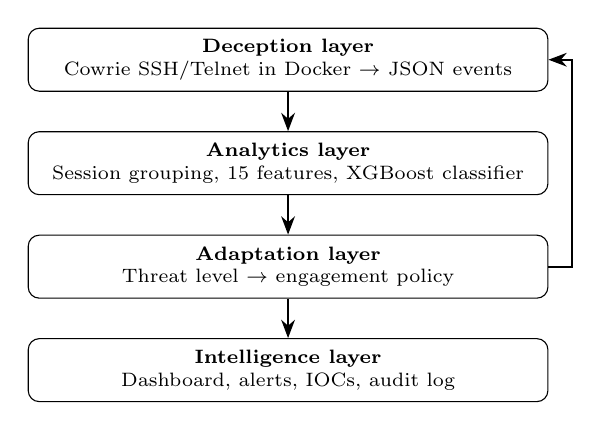
\begin{tikzpicture}[box/.style={draw,rounded corners,minimum width=6.6cm,minimum height=0.8cm,align=center,font=\scriptsize},
  arr/.style={-{Stealth},thick}, node distance=0.5cm]
\node[box] (d) {\textbf{Deception layer}\\Cowrie SSH/Telnet in Docker $\rightarrow$ JSON events};
\node[box,below=of d] (a) {\textbf{Analytics layer}\\Session grouping, 15 features, XGBoost classifier};
\node[box,below=of a] (r) {\textbf{Adaptation layer}\\Threat level $\rightarrow$ engagement policy};
\node[box,below=of r] (i) {\textbf{Intelligence layer}\\Dashboard, alerts, IOCs, audit log};
\draw[arr] (d) -- (a); \draw[arr] (a) -- (r); \draw[arr] (r) -- (i);
\draw[arr] (r.east) -- ++(0.3,0) |- (d.east);
\end{tikzpicture}
\caption{\sys\ four-layer architecture. The feedback arrow carries the engagement policy back to the honeypot.}
\label{fig:arch}
\end{figure}

\subsection{Deception Layer: Cowrie}
Cowrie is chosen because it emulates SSH and Telnet, records sessions as JSON, and can run in an isolated Docker container; it is the deception base in \cite{ref1,ref2,ref5}. The honeypot is deployed with no route to production networks, and outbound traffic is blocked by default (see the Kill Switch in Section~\ref{sec:resp}). Each connection yields a session identifier, and events such as login attempts, command input, file downloads, file uploads, and session close are logged against it.

\subsection{Analytics Layer: Feature Extraction}\label{sec:feat}
Each session is represented by 15 features: ten at session level (Table~\ref{tab:sess}) and five at payload level (Table~\ref{tab:pay}). Numeric features are standardized using statistics fitted on the training split only. Sessions with no commands (e.g., authentication-only probes) receive zero for count-based features and a sentinel value for timing features, which gradient-boosted trees handle natively. Feature choices follow the behavioral signals discussed in \cite{ref1,ref4}; their individual contribution is to be tested in the ablation study (Section~\ref{sec:ablation}).

\begin{figure*}[t]
\centering
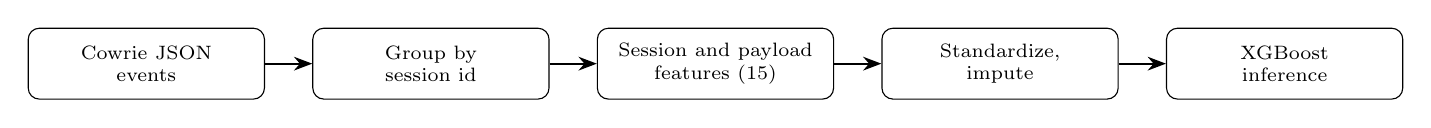
\begin{tikzpicture}[box/.style={draw,rounded corners,minimum width=3cm,minimum height=0.9cm,align=center,font=\scriptsize},
  arr/.style={-{Stealth},thick}, node distance=0.6cm]
\node[box] (a) {Cowrie JSON\\events};
\node[box,right=of a] (b) {Group by\\session id};
\node[box,right=of b] (c) {Session and payload\\features (15)};
\node[box,right=of c] (d) {Standardize,\\impute};
\node[box,right=of d] (e) {XGBoost\\inference};
\foreach \x/\y in {a/b,b/c,c/d,d/e} \draw[arr] (\x) -- (\y);
\end{tikzpicture}
\caption{Feature extraction pipeline from raw Cowrie events to a threat-level prediction.}
\label{fig:pipe}
\end{figure*}

\begin{table}[t]
\centering
\caption{Session-Level Features}
\label{tab:sess}
\footnotesize
\begin{tabular}{@{}p{2.9cm}p{5.3cm}@{}}
\toprule
Feature & Definition \\
\midrule
\texttt{command\_\allowbreak{}count} & Number of commands entered \\
\texttt{command\_\allowbreak{}diversity} & Unique commands divided by total commands \\
\texttt{inter\_\allowbreak{}command\_\allowbreak{}delay\_\allowbreak{}avg} & Mean time between consecutive commands \\
\texttt{session\_\allowbreak{}duration} & Time from connect to close \\
\texttt{download\_\allowbreak{}attempts} & Count of file-download events or download commands \\
\texttt{privilege\_\allowbreak{}escalation} & Count of commands matching a privilege-escalation pattern list \\
\texttt{lateral\_\allowbreak{}movement} & Count of commands that target other hosts (pattern list) \\
\texttt{file\_\allowbreak{}upload\_\allowbreak{}count} & Count of file-upload events \\
\texttt{unique\_\allowbreak{}commands} & Absolute count of distinct commands \\
\texttt{failed\_\allowbreak{}auth\_\allowbreak{}attempts} & Count of failed login events \\
\bottomrule
\end{tabular}
\end{table}

\begin{table}[t]
\centering
\caption{Payload-Level Features}
\label{tab:pay}
\footnotesize
\begin{tabular}{@{}p{2.9cm}p{5.3cm}@{}}
\toprule
Feature & Definition \\
\midrule
\texttt{command\_\allowbreak{}length\_\allowbreak{}avg} & Mean character length of commands \\
\texttt{entropy\_\allowbreak{}score} & Mean Shannon entropy of command strings \\
\texttt{base64\_\allowbreak{}presence} & Count of commands containing base64-like blobs \\
\texttt{known\_\allowbreak{}malicious\_\allowbreak{}signatures} & Count of commands matching a signature list \\
\texttt{threat\_\allowbreak{}db\_\allowbreak{}matches} & Count of URLs/IPs/hashes found in a threat-intelligence source \\
\bottomrule
\end{tabular}
\end{table}

\subsection{Classification Layer: XGBoost}\label{sec:clf}
XGBoost \cite{ref13} is selected for three reasons: it handles tabular features with mixed scales, supports class weighting and custom objectives for imbalance, and offers fast inference and feature-importance output. Cowrie-based systems in \cite{ref1,ref2} use the same model family. Whether XGBoost outperforms RF \cite{ref4,ref5} on this task is an empirical question addressed in Section~\ref{sec:eval}.

\textbf{Label derivation (heuristic).} The Shell Honeypot dataset \cite{ref10} annotates commands with a severity index $V_i\in[0,4]$ and does not provide the three threat classes used here. We therefore \emph{derive} labels with the rule in Table~\ref{tab:label}. Since $V_i$ is defined per command, a session-level label requires aggregation; we use the maximum $V_i$ over a session's commands, so a session is labeled by its most severe action. \ver{confirm that the dataset exposes session identifiers or an ordering from which sessions can be reconstructed; if not, label per command window instead and revise Table~\ref{tab:sess} accordingly}. The thresholds are design choices, not empirical findings, and a sensitivity analysis over alternative thresholds is part of the protocol.

\begin{table}[t]
\centering
\caption{Label Derivation Rule (Heuristic)}
\label{tab:label}
\footnotesize
\begin{tabular}{@{}lll@{}}
\toprule
Severity range & Class & Interpretation \\
\midrule
$V_i<1.5$ & Scanner & Automated, low sophistication \\
$1.5\le V_i<3.0$ & Amateur & Semi-skilled, script-based \\
$V_i\ge 3.0$ & Advanced & Skilled, multi-stage activity \\
\bottomrule
\end{tabular}
\end{table}

\textbf{Class imbalance.} Scanner sessions are expected to dominate real honeypot traffic. Following \cite{ref2}, we will evaluate a focal-loss objective, which down-weights easy examples by a factor $(1-p_t)^\gamma$:
\begin{equation}
\mathcal{L}_{\text{focal}} = -\alpha_t\,(1-p_t)^{\gamma}\,\log(p_t),
\end{equation}
where $p_t$ is the predicted probability of the true class. The focusing parameter $\gamma$ and class weights $\alpha_t$ are tuned on validation data; plain class-weighted cross-entropy serves as the comparison.

\subsection{Adaptation Layer: Response Engine}\label{sec:resp}
The response engine maps the predicted level to an engagement policy. The values below are \emph{initial design choices} to be tuned, and the effects attributed to them are hypotheses (Section~\ref{sec:hyp}), not findings.
\begin{itemize}
\item \textbf{Scanner:} log only, minimal interaction, short timeout (initial value: 5 min). \emph{Hypothesis:} saves resources without reducing useful intelligence.
\item \textbf{Amateur:} standard engagement, capture all commands and downloads, session timeout of 30 min (initial value). \emph{Hypothesis:} yields richer command and payload capture than a Scanner policy.
\item \textbf{Advanced:} maximum engagement, extended fake filesystem content and service responses, containment controls active. \emph{Hypothesis:} prolongs engagement and increases IOCs per session.
\end{itemize}
\textbf{Escalation and de-escalation.} Classification is repeated as a session unfolds (e.g., after every $k$ commands, with $k$ a tunable parameter). A session may move up one level when new evidence raises the predicted class, and moves down only after a configurable number of consecutive lower predictions, to avoid oscillation.

\textbf{Kill Switch.} The Kill Switch is a containment mechanism, not an engagement mechanism. It terminates a session and blocks its source when predefined safety conditions hold, such as attempted outbound connections, resource exhaustion by an automated client, or exceeding a hard session limit. The idea of separating bot-like from human-like behavior is motivated by the bot-versus-human classifier in \cite{ref6}; the specific triggers here are our design.

\subsection{Intelligence Layer: Dashboard}
The dashboard presents a live attack feed, threat-level distribution, top source IP addresses, per-session timelines, and extracted IOCs. Real-time alerting with a Flask dashboard follows \cite{ref5}. Reference~\cite{ref6} reports visualization latency under 120\,ms; we adopt this as a comparison point and will measure our own latency rather than assume it (Section~\ref{sec:setup}).

\section{Implementation}\label{sec:impl}
\subsection{Technology Stack}
The prototype uses Python 3.10 or later; Cowrie in Docker; XGBoost, scikit-learn, pandas, and NumPy for modeling; FastAPI for a classification endpoint; Flask or Streamlit for the dashboard; and SQLite (PostgreSQL for larger deployments) for storage. \ver{pin exact library versions used in the final experiments}

\subsection{Dataset}\label{sec:dataset}
Training and evaluation will use the Shell Honeypot Attack Request--Response dataset \cite{ref10} (12,923 commands from 2021--22 and 4,236 from 2024). Because that dataset consists of command and response records, timing and authentication features in Table~\ref{tab:sess} may be unavailable for it. Two options are planned: restrict the feature set to those derivable from the data, or collect sessions from our own Cowrie deployment over a period of several weeks. MURHCAD \cite{ref11} (132,425 events, 2,438 unique IPs, 95 countries) is a candidate for supplementary Cowrie sessions. \tbf{final dataset used, session counts per class after labeling}

\subsection{Feature Extraction Pipeline}
Listing~\ref{lst:feat} shows the core of session-level extraction from Cowrie JSON events. Pattern lists for privilege escalation and lateral movement are illustrative and will be published with the repository.

\begin{lstlisting}[float=t,caption={Session feature extraction (excerpt).},label={lst:feat}]
import json, math, re
from collections import Counter, defaultdict
from datetime import datetime

PRIV = re.compile(r"\b(sudo|su\s|chmod\s+\+s)")

def entropy(s):
    c = Counter(s)
    n = len(s) or 1
    return -sum(v/n * math.log2(v/n) for v in c.values())

def load_sessions(path):
    sessions = defaultdict(list)
    with open(path) as f:
        for line in f:
            e = json.loads(line)
            sessions[e["session"]].append(e)
    return sessions

def features(events):
    parse_ts = lambda e: datetime.fromisoformat(
        e["timestamp"].replace("Z", "+00:00"))
    cmds = [e for e in events
            if e["eventid"] == "cowrie.command.input"]
    text = [e["input"] for e in cmds]
    ts = [parse_ts(e) for e in cmds]
    gaps = [(b - a).total_seconds() for a, b in zip(ts, ts[1:])]
    return {
        "command_count": len(text),
        "unique_commands": len(set(text)),
        "command_diversity": len(set(text)) / max(len(text), 1),
        "inter_command_delay_avg": sum(gaps) / len(gaps) if gaps else -1,
        "failed_auth_attempts": sum(
            e["eventid"] == "cowrie.login.failed" for e in events),
        "privilege_escalation": sum(bool(PRIV.search(x)) for x in text),
        "entropy_score": sum(map(entropy, text)) / max(len(text), 1),
    }
\end{lstlisting}

\subsection{Model Training}\label{sec:training}
Table~\ref{tab:hp} lists the hyperparameters. These are initial \emph{choices}, not tuned results. Data is split 80/20 with stratification by class; model selection uses 5-fold stratified cross-validation on the training portion, with early stopping on a validation fold. Grid search over the ranges in Table~\ref{tab:hp} precedes the final fit, and the test split is used once.

\begin{table}[t]
\centering
\caption{XGBoost Hyperparameters (Design Choices)}
\label{tab:hp}
\footnotesize
\begin{tabular}{@{}p{2.6cm}p{1.6cm}p{3.9cm}@{}}
\toprule
Parameter & Initial & Grid search range \\
\midrule
\texttt{max\_\allowbreak{}depth} & 6 & \{4, 6, 8\} \\
\texttt{learning\_\allowbreak{}rate} & 0.1 & \{0.05, 0.1, 0.2\} \\
\texttt{n\_\allowbreak{}estimators} & 100 & \{100, 200, 300\} \\
Early stopping rounds & 10 & fixed \\
Objective & softprob & softprob vs.\ focal loss \\
Focal $\gamma$ & --- & \tbf{range} \\
\bottomrule
\end{tabular}
\end{table}

\subsection{Adaptive Response Implementation}
The response engine is a rule table keyed by predicted class, read by a small service that adjusts Cowrie parameters (session timeout, filesystem profile) and invokes container-level controls for the Kill Switch. \ver{confirm which Cowrie configuration options can be changed per session at runtime versus requiring a restart; if per-session changes are not supported, implement the policy through a proxy or a custom Cowrie output/command plugin}.

\subsection{Dashboard Implementation}
A Flask service reads from the session database and serves a JSON API consumed by the page, which polls or subscribes for updates. Alerts are generated when a session reaches the Advanced class or triggers the Kill Switch.

\subsection{Reproducibility}
Code, pattern lists, labeling script, and configuration will be released in a public repository. \tbf{repository URL}

\section{Evaluation Protocol}\label{sec:eval}
This section specifies what will be measured. No results are reported in this draft.

\subsection{Experimental Setup}\label{sec:setup}
Experiments will use the dataset(s) of Section~\ref{sec:dataset} with the stratified 80/20 split and 5-fold cross-validation of Section~\ref{sec:training}. \tbf{hardware} and \tbf{exact software versions}. Engagement experiments require live or replayed attacker sessions against two deployments: a static Cowrie configuration and \sys. Classification latency and dashboard latency are measured end to end.

\subsection{Hypotheses}\label{sec:hyp}
\begin{itemize}
\item \textbf{H1:} Adaptive deception increases mean engagement duration compared with a static Cowrie configuration.
\item \textbf{H2:} XGBoost achieves accuracy above 95\% on the derived three-class problem. This is a target, and its success depends in part on the labeling heuristic (Section~\ref{sec:validity}).
\item \textbf{H3:} Threat-level-specific responses improve threat-intelligence quality, measured as IOCs per session and MITRE ATT\&CK technique coverage.
\end{itemize}

\subsection{Metrics}
\emph{Classification:} accuracy, per-class precision, recall, and F1, and weighted and macro averages; confusion matrix. \emph{Engagement:} mean and median session duration and commands per session. \emph{Intelligence quality:} count of unique IOCs (IPs, URLs, hashes) per session and the number of distinct MITRE ATT\&CK techniques \cite{ref15} observed. \emph{Efficiency:} inference latency and dashboard update latency.

\subsection{Baselines}
(1) Static Cowrie with a fixed policy; (2) a rule-based classifier using thresholds on command count and signature matches; (3) Random Forest on the same features, motivated by \cite{ref4,ref5}.

\subsection{Comparison Table}
Table~\ref{tab:cmp} lists reported figures from prior work next to \sys\ placeholders. Prior figures are quoted as reported by their sources and \emph{are not directly comparable}: tasks, datasets, and metrics differ (e.g., \cite{ref4} uses NSL-KDD, and \cite{ref3} reports detection rather than three-class accuracy).

\begin{table}[t]
\centering
\caption{Comparison with Reported Figures}
\label{tab:cmp}
\footnotesize
\begin{tabular}{@{}p{1.4cm}p{4.7cm}p{1.1cm}@{}}
\toprule
System & Reported metric & Source \\
\midrule
Static Cowrie & \tbf{our measurement} & ours \\
Rule-based & \tbf{our measurement} & ours \\
Random Forest & \tbf{our measurement}; \cite{ref4}: 17,354 TP, 235 FN, 196 FP (NSL-KDD) & ours; \cite{ref4} \\
RL honeypot & 97\% detection accuracy, 3.8\% FP & \cite{ref3} \\
RL+LLM & +23\% engagement reward; +55 pp intent accuracy vs.\ Wazuh & \cite{ref9} \\
HoneyTrap & 100\% credential capture; $<$120\,ms visualization & \cite{ref6} \\
GMNH & Not reported in \cite{ref2} & \cite{ref2} \\
Asgard2.0 & Not reported in \cite{ref7} & \cite{ref7} \\
\textbf{Proposed} & \tbf{accuracy, F1, engagement, IOCs/session} & ours \\
\bottomrule
\end{tabular}
\end{table}

\begin{figure}[t]
\centering
% Replace with: \includegraphics[width=\columnwidth]{figures/FILENAME.png}
% Generated by: python src/evaluator.py --plot confusion
\fbox{\parbox{0.9\columnwidth}{\centering\vspace{1.2cm}\tbf{confusion matrix; generate after experiments}\vspace{1.2cm}}}
\caption{Confusion matrix of the XGBoost classifier on the test split.}
\label{fig:cm}
\end{figure}

\begin{figure}[t]
\centering
% Replace with: \includegraphics[width=\columnwidth]{figures/FILENAME.png}
% Generated by: python src/evaluator.py --plot comparison
\fbox{\parbox{0.9\columnwidth}{\centering\vspace{1.2cm}\tbf{baseline comparison chart; generate after experiments}\vspace{1.2cm}}}
\caption{Comparison of \sys\ with baselines on accuracy, F1, and engagement duration.}
\label{fig:cmp}
\end{figure}

\subsection{Ablation Study}\label{sec:ablation}
The following variants will be run under the same split: (a) without the adaptation layer (classification only); (b) without the payload-level feature group; (c) leave-one-feature-group-out over session-level features; (d) Random Forest in place of XGBoost; (e) focal loss versus weighted cross-entropy; (f) alternative $V_i$ thresholds for the label rule. \tbf{results for each variant}

\subsection{Threats to Validity}\label{sec:validity}
\emph{Label circularity.} Labels derive from $V_i$, and features such as signature matches may correlate with $V_i$ by construction; high accuracy could partly reflect the labeling rule rather than real attacker skill. We will report results with signature-based features removed. \emph{Dataset age and drift.} The commands in \cite{ref10} span 2021--22 and 2024, and attacker behavior changes over time; we will test training on one period and evaluating on the other. \emph{Lab versus production.} Controlled evaluations can overstate production performance \cite{ref1}; live deployment is future work. \emph{Dataset provenance.} Results on one dataset may not transfer to others such as \cite{ref11}.

\section{Discussion}\label{sec:disc}
\subsection{Design Implications}
If the hypotheses hold, a continuously updated threat estimate lets defenders allocate engagement where it yields intelligence and contain risk where it does not. For security operations teams, a three-level output is simple to act on. For researchers, an explicit labeling rule and published code make comparison and criticism possible. Whether three classes are sufficient is itself a question the ablations and threshold-sensitivity analysis will inform.

\subsection{Limitations}
The framework inherits the lab-versus-production gap noted in \cite{ref1}. The labeling heuristic is not validated against expert annotation, and session-level aggregation of a command-level severity index is a simplification. Pattern lists for privilege escalation and lateral movement are incomplete by nature. Scalability to many concurrent sessions has not been assessed.

\subsection{Attacker Adaptation}
Attackers may use automated tools, including AI-based techniques, to recognize honeypots \cite{ref8}. A response engine that behaves deterministically per class could itself become a fingerprint. Randomizing parts of the policy and incorporating learned response generation as in \cite{ref8} are directions to explore.

\subsection{Ethical Considerations}
Operating a honeypot raises legal and privacy questions that vary by jurisdiction, including the handling of source IP addresses and attacker-supplied data. The Kill Switch and outbound filtering exist to prevent the system from being used to harm third parties. Collected data should be stored securely and shared only in a minimized form, and any disclosure of discovered malware or infrastructure should follow responsible-disclosure practice.

\section{Conclusion and Future Work}\label{sec:concl}
\subsection{Summary}
This draft presented \sys, a four-layer framework that links session-level threat classification with adaptive engagement in a Cowrie-based honeypot. We specified a 15-feature representation, an XGBoost classifier with optional focal loss, an explicit heuristic that derives Scanner, Amateur, and Advanced labels from the severity index of an existing dataset, and a response engine with a containment Kill Switch. We also defined an evaluation protocol with three hypotheses, baselines, and ablations. The experiments remain to be run, and the paper's claims will be set by their outcome.

\subsection{Future Work}
Planned directions are: reinforcement-learning-based response selection in the spirit of \cite{ref7}; LLM-generated deceptive responses as explored in \cite{ref9}; federated learning across distributed honeypots; production deployment with long-term monitoring; and support for additional protocols beyond SSH and Telnet, such as HTTP, FTP, and SQL \cite{ref6}.

\section*{Acknowledgment}
The authors thank PRAM Educate IT Software LLP for their support.

% NOTE: Refs [1]-[12] and [16] require verification against IEEE Xplore,
% ACM DL, or arXiv before submission. Replace all [VERIFY: ...] fields.
% Do not submit with placeholder text.
\begin{thebibliography}{99}
\bibitem{ref1} ``AI-Assisted Honeypot for Threat Adaptation and Mitigation,'' IEEE, Mar. 2026. \ver{authors, venue, DOI}
\bibitem{ref2} ``GhostMesh Neuro-Honeynet (GMNH),'' IEEE, Feb. 2026. \ver{authors, venue, DOI}
\bibitem{ref3} ``A Dynamic AI-Powered Honeypot Framework,'' IEEE, Oct. 2025. \ver{authors, venue, DOI}
\bibitem{ref4} ``Adaptive Honeypot Simulation \& Intrusion Detection Using Supervised ML,'' IEEE, Nov. 2025. \ver{authors, venue, DOI}
\bibitem{ref5} ``Forensic Analysis of AI-Driven Cyber Deception Networks,'' Zenodo, May 2026. \ver{authors, DOI}
\bibitem{ref6} ``HoneyTrap: AI-Powered Honeypot for Cyberattack Detection,'' IJERT, 2026. \ver{authors, volume, pages}
\bibitem{ref7} ``Asgard2.0: Adaptive Self-Guarded Risk-Aware Honeypot Using DRL,'' ACM ESORICS 2025. \ver{authors, pages, DOI}
\bibitem{ref8} ``Q-Cowrie: An Adaptive Honeypot,'' ACM IJIS, Feb. 2026. \ver{authors, volume, pages, DOI}
\bibitem{ref9} ``Reinforcement Learning Meets LLM Honeypots,'' IEEE, Sep. 2026. \ver{authors, venue, DOI}
\bibitem{ref10} ``Shell Honeypot Attack Request--Response Dataset,'' HuggingFace. \ver{authors, year, DOI}
\bibitem{ref11} ``MURHCAD: Multi-Regional Cloud Honeypot Dataset,'' arXiv, 2026. \ver{authors, DOI}
\bibitem{ref12} ``SoK: Honeypots \& LLMs,'' IEEE, 2026. \ver{authors, venue, DOI}
\bibitem{ref13} T. Chen and C. Guestrin, ``XGBoost: A scalable tree boosting system,'' in \emph{Proc. 22nd ACM SIGKDD Int. Conf. Knowl. Discovery Data Mining}, 2016, pp. 785--794.
\bibitem{ref14} M. Tavallaee, E. Bagheri, W. Lu, and A. A. Ghorbani, ``A detailed analysis of the KDD CUP 99 data set,'' in \emph{Proc. IEEE Symp. Comput. Intell. Secur. Defense Appl.}, 2009.
\bibitem{ref15} B. Strom \emph{et al.}, ``MITRE ATT\&CK: Design and philosophy,'' MITRE Tech. Rep., 2018.
\bibitem{ref16} M. Oosterhof, ``Cowrie SSH/Telnet honeypot,'' GitHub repository. \ver{URL, access date}
\end{thebibliography}

\balance
\end{document}
